\begin{figure*}[t]
	\centering
	
	\subfloat[EPICA rack: from left to right: the power supply, the timing module, the control module and eight probe modules.]{
		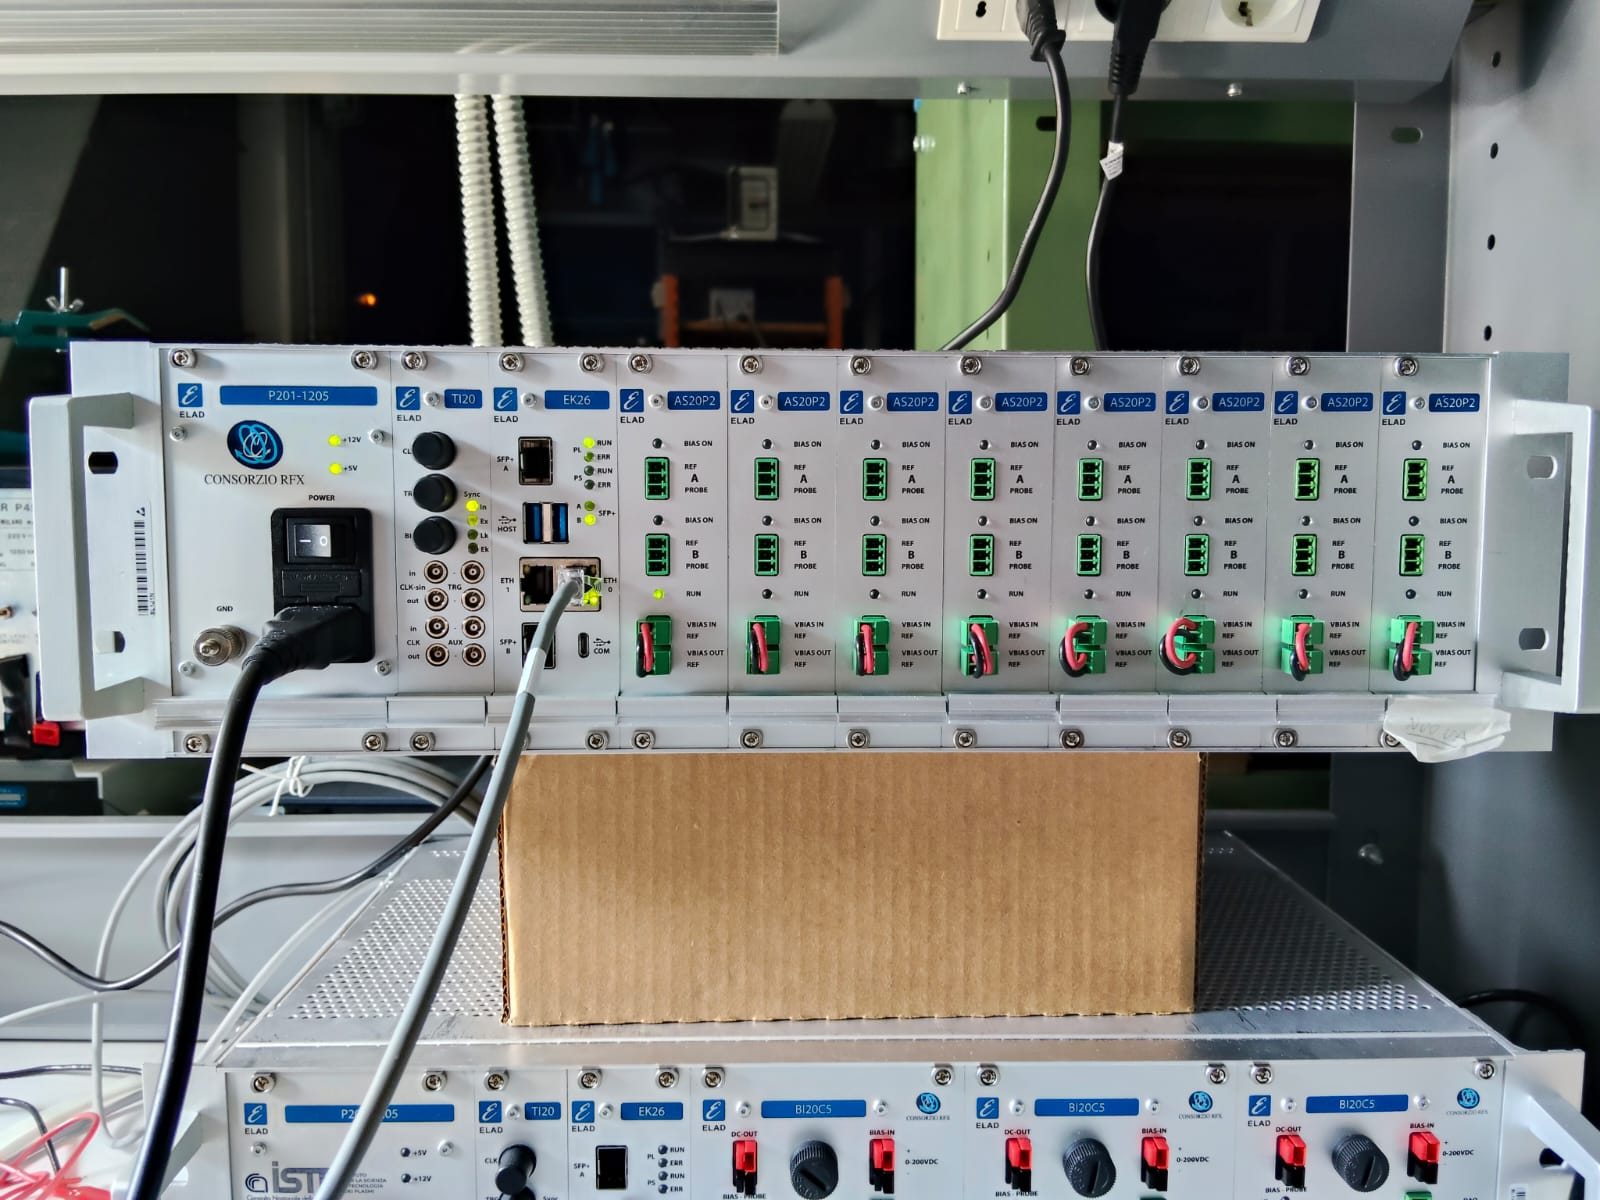
\includegraphics[width=3.2in]{epica}
		\label{fig3a}
	}
	\hfill
	\subfloat[Integrated probe management module, including biasing and signal conditioning stages.]{
		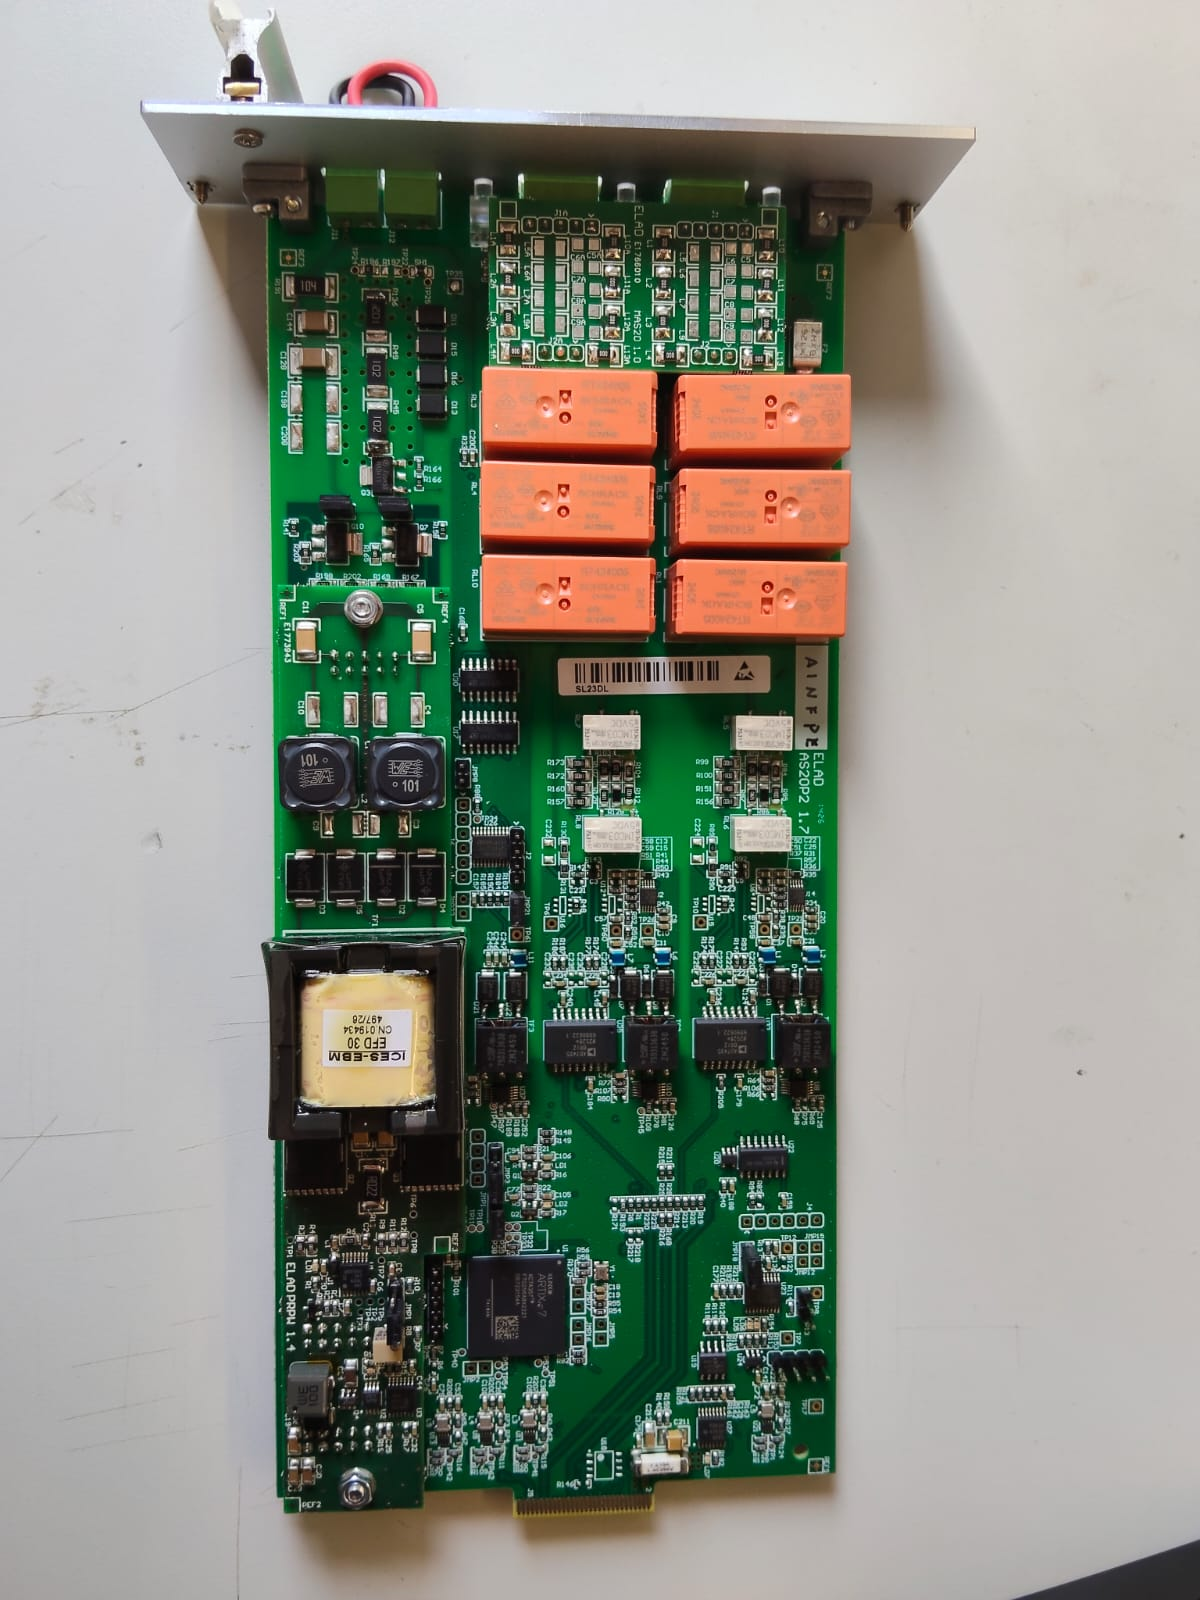
\includegraphics[width=2.3in,angle=90]{epica_module}
		\label{fig3b}
	}
	\vspace{0.5cm}
	\subfloat[Epica internal system overview.]{
		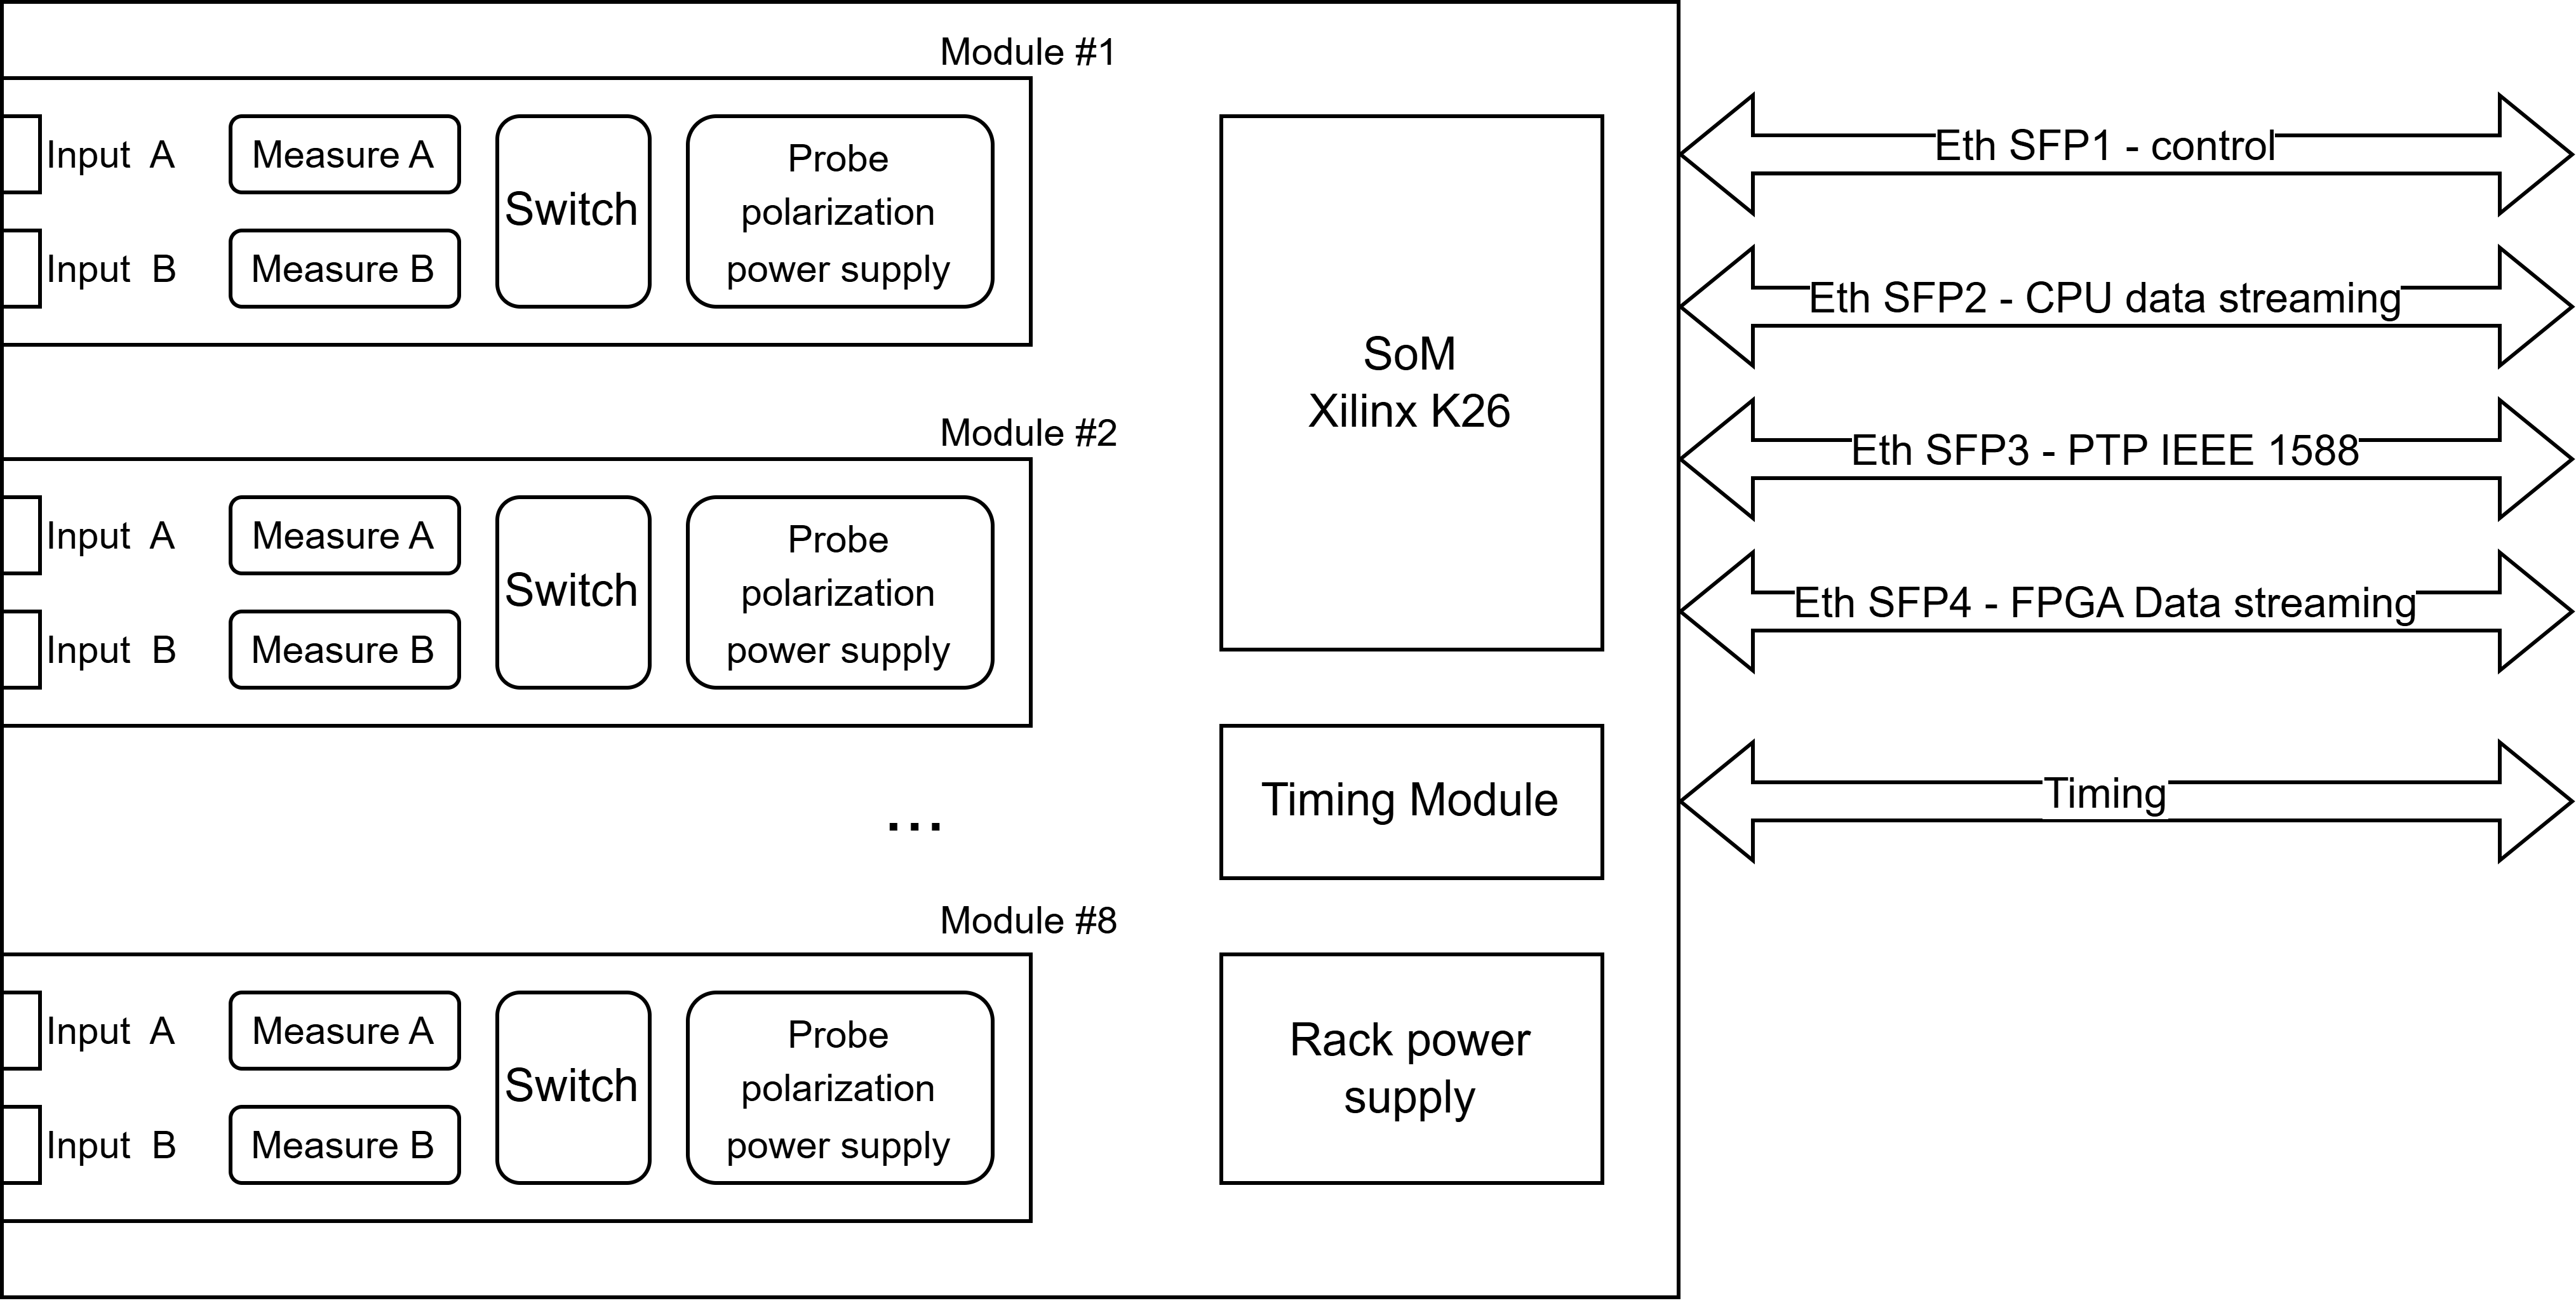
\includegraphics[width=4in]{epica_int4}
		\label{fig3c}
	}
	
	\caption{EPICA housing, probe management module and system overview.}
	\label{fig3}
\end{figure*}

Fig.~\ref{fig3a} shows the rack enclosure hosting the complete system, whereas Fig.~\ref{fig3c} illustrates the internal system overview. The platform supports up to 16 probes, arranged into eight electrically and functionally independent probe pairs. Each pair is managed by a dedicated acquisition and biasing module responsible for electrode polarization and signal acquisition. This modular organization enables straightforward system expansion while maintaining electrical isolation and operational flexibility, making EPICA suitable for a broad range of plasma diagnostics applications.

The system consists of four main subsystems: the power supply unit, the timing module, the controller module, and probe modules.

The power supply unit generates the primary \measure{5}{V} and \measure{12}{V} DC rails distributed throughout the system. Additional voltage levels required by individual subsystems are generated locally through dedicated DC/DC converters integrated within each module, ensuring proper electrical isolation both between modules and among different functional sections of the same module. This distributed power architecture also mitigates ground-loop effects.

The timing module provides the synchronization reference for both the controller and probe modules. It can operate either as a standalone timing source or be connected to an external master clock, enabling synchronization with other diagnostics and consistent temporal correlation of measurements. Alternatively, when Precision Time Protocol (PTP) synchronization is adopted, timing information is distributed through the Ethernet network, eliminating the need for a dedicated timing module. In this configuration, the PTP interface is implemented within the controller module.

To support integrated probe biasing, real-time data streaming and high-resolution acquisition, EPICA relies on a high-performance controller platform based on the KRIA K26 SoM \cite{KRIA}. The selected platform combines an FPGA with a quad-core ARM processor within the same chip, enabling tight integration between deterministic real-time control and high-throughput data processing.

Communication between modules is carried out using the back panel bus. It consists of Low Voltage Differential Signal (LVDS) rails for clock distribution and data exchange, and DC power rails for power transmission.

The system software is implemented using the MARTe2 \cite{manduchi} real-time framework, executed on the embedded processor to manage supervisory control, and communication tasks. Time-critical functions, including low-latency signal acquisition and preprocessing, are implemented within the FPGA. 

The probe modules implement the analog front-end electronics, probe bias generation, signal conditioning, and analog-to-digital conversion. Digitized measurements are transmitted to the controller via LVDS rails of the back panel bus for further processing, storage, and streaming.

Communication between EPICA and external systems is performed through Ethernet interfaces, available on the controller, as illustrated in Fig.~\ref{fig3c}, enabling simultaneous data streaming, synchronization, and integration with supervisory frameworks. In addition, a USB serial console is provided for system configuration, firmware deployment and debugging.